% Created by tikzDevice version 0.10.1 on 2016-09-10 14:28:55
% !TEX encoding = UTF-8 Unicode
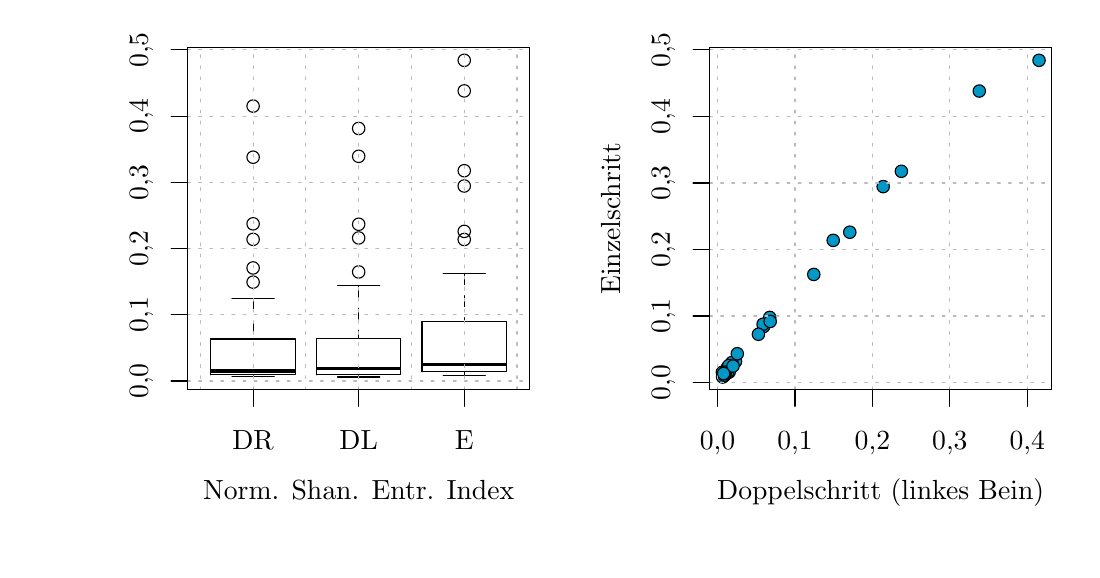
\begin{tikzpicture}[x=1pt,y=1pt]
\definecolor{fillColor}{RGB}{255,255,255}
\path[use as bounding box,fill=fillColor,fill opacity=0.00] (0,0) rectangle (377.25,188.62);
\begin{scope}
\path[clip] ( 57.82, 57.82) rectangle (181.40,181.40);
\definecolor{drawColor}{RGB}{0,0,0}

\path[draw=drawColor,line width= 1.2pt,line join=round] ( 66.21, 64.53) -- ( 96.72, 64.53);

\path[draw=drawColor,line width= 0.4pt,dash pattern=on 4pt off 4pt ,line join=round,line cap=round] ( 81.46, 62.42) -- ( 81.46, 63.18);

\path[draw=drawColor,line width= 0.4pt,dash pattern=on 4pt off 4pt ,line join=round,line cap=round] ( 81.46, 90.67) -- ( 81.46, 76.12);

\path[draw=drawColor,line width= 0.4pt,line join=round,line cap=round] ( 73.84, 62.42) -- ( 89.09, 62.42);

\path[draw=drawColor,line width= 0.4pt,line join=round,line cap=round] ( 73.84, 90.67) -- ( 89.09, 90.67);

\path[draw=drawColor,line width= 0.4pt,line join=round,line cap=round] ( 66.21, 63.18) --
	( 96.72, 63.18) --
	( 96.72, 76.12) --
	( 66.21, 76.12) --
	( 66.21, 63.18);

\path[draw=drawColor,line width= 0.4pt,line join=round,line cap=round] ( 81.46,101.80) circle (  2.25);

\path[draw=drawColor,line width= 0.4pt,line join=round,line cap=round] ( 81.46, 96.67) circle (  2.25);

\path[draw=drawColor,line width= 0.4pt,line join=round,line cap=round] ( 81.46,112.12) circle (  2.25);

\path[draw=drawColor,line width= 0.4pt,line join=round,line cap=round] ( 81.46,141.81) circle (  2.25);

\path[draw=drawColor,line width= 0.4pt,line join=round,line cap=round] ( 81.46,160.28) circle (  2.25);

\path[draw=drawColor,line width= 0.4pt,line join=round,line cap=round] ( 81.46,117.74) circle (  2.25);

\path[draw=drawColor,line width= 1.2pt,line join=round] (104.35, 65.35) -- (134.86, 65.35);

\path[draw=drawColor,line width= 0.4pt,dash pattern=on 4pt off 4pt ,line join=round,line cap=round] (119.61, 62.39) -- (119.61, 63.14);

\path[draw=drawColor,line width= 0.4pt,dash pattern=on 4pt off 4pt ,line join=round,line cap=round] (119.61, 95.30) -- (119.61, 76.40);

\path[draw=drawColor,line width= 0.4pt,line join=round,line cap=round] (111.98, 62.39) -- (127.24, 62.39);

\path[draw=drawColor,line width= 0.4pt,line join=round,line cap=round] (111.98, 95.30) -- (127.24, 95.30);

\path[draw=drawColor,line width= 0.4pt,line join=round,line cap=round] (104.35, 63.14) --
	(134.86, 63.14) --
	(134.86, 76.40) --
	(104.35, 76.40) --
	(104.35, 63.14);

\path[draw=drawColor,line width= 0.4pt,line join=round,line cap=round] (119.61,100.35) circle (  2.25);

\path[draw=drawColor,line width= 0.4pt,line join=round,line cap=round] (119.61,112.64) circle (  2.25);

\path[draw=drawColor,line width= 0.4pt,line join=round,line cap=round] (119.61,142.14) circle (  2.25);

\path[draw=drawColor,line width= 0.4pt,line join=round,line cap=round] (119.61,152.20) circle (  2.25);

\path[draw=drawColor,line width= 0.4pt,line join=round,line cap=round] (119.61,117.58) circle (  2.25);

\path[draw=drawColor,line width= 1.2pt,line join=round] (142.49, 66.86) -- (173.01, 66.86);

\path[draw=drawColor,line width= 0.4pt,dash pattern=on 4pt off 4pt ,line join=round,line cap=round] (157.75, 62.95) -- (157.75, 64.28);

\path[draw=drawColor,line width= 0.4pt,dash pattern=on 4pt off 4pt ,line join=round,line cap=round] (157.75, 99.82) -- (157.75, 82.43);

\path[draw=drawColor,line width= 0.4pt,line join=round,line cap=round] (150.12, 62.95) -- (165.38, 62.95);

\path[draw=drawColor,line width= 0.4pt,line join=round,line cap=round] (150.12, 99.82) -- (165.38, 99.82);

\path[draw=drawColor,line width= 0.4pt,line join=round,line cap=round] (142.49, 64.28) --
	(173.01, 64.28) --
	(173.01, 82.43) --
	(142.49, 82.43) --
	(142.49, 64.28);

\path[draw=drawColor,line width= 0.4pt,line join=round,line cap=round] (157.75,115.01) circle (  2.25);

\path[draw=drawColor,line width= 0.4pt,line join=round,line cap=round] (157.75,112.08) circle (  2.25);

\path[draw=drawColor,line width= 0.4pt,line join=round,line cap=round] (157.75,131.41) circle (  2.25);

\path[draw=drawColor,line width= 0.4pt,line join=round,line cap=round] (157.75,165.77) circle (  2.25);

\path[draw=drawColor,line width= 0.4pt,line join=round,line cap=round] (157.75,176.82) circle (  2.25);

\path[draw=drawColor,line width= 0.4pt,line join=round,line cap=round] (157.75,136.93) circle (  2.25);
\end{scope}
\begin{scope}
\path[clip] (  0.00,  0.00) rectangle (377.25,188.62);
\definecolor{drawColor}{RGB}{0,0,0}

\path[draw=drawColor,line width= 0.4pt,line join=round,line cap=round] ( 81.46, 57.82) -- (157.75, 57.82);

\path[draw=drawColor,line width= 0.4pt,line join=round,line cap=round] ( 81.46, 57.82) -- ( 81.46, 51.82);

\path[draw=drawColor,line width= 0.4pt,line join=round,line cap=round] (119.61, 57.82) -- (119.61, 51.82);

\path[draw=drawColor,line width= 0.4pt,line join=round,line cap=round] (157.75, 57.82) -- (157.75, 51.82);

\node[text=drawColor,anchor=base,inner sep=0pt, outer sep=0pt, scale=  1.00] at ( 81.46, 36.22) {DR};

\node[text=drawColor,anchor=base,inner sep=0pt, outer sep=0pt, scale=  1.00] at (119.61, 36.22) {DL};

\node[text=drawColor,anchor=base,inner sep=0pt, outer sep=0pt, scale=  1.00] at (157.75, 36.22) {E};

\path[draw=drawColor,line width= 0.4pt,line join=round,line cap=round] ( 57.82, 60.94) -- ( 57.82,180.58);

\path[draw=drawColor,line width= 0.4pt,line join=round,line cap=round] ( 57.82, 60.94) -- ( 51.82, 60.94);

\path[draw=drawColor,line width= 0.4pt,line join=round,line cap=round] ( 57.82, 84.87) -- ( 51.82, 84.87);

\path[draw=drawColor,line width= 0.4pt,line join=round,line cap=round] ( 57.82,108.80) -- ( 51.82,108.80);

\path[draw=drawColor,line width= 0.4pt,line join=round,line cap=round] ( 57.82,132.72) -- ( 51.82,132.72);

\path[draw=drawColor,line width= 0.4pt,line join=round,line cap=round] ( 57.82,156.65) -- ( 51.82,156.65);

\path[draw=drawColor,line width= 0.4pt,line join=round,line cap=round] ( 57.82,180.58) -- ( 51.82,180.58);

\node[text=drawColor,rotate= 90.00,anchor=base,inner sep=0pt, outer sep=0pt, scale=  1.00] at ( 43.42, 60.94) {0,0};

\node[text=drawColor,rotate= 90.00,anchor=base,inner sep=0pt, outer sep=0pt, scale=  1.00] at ( 43.42, 84.87) {0,1};

\node[text=drawColor,rotate= 90.00,anchor=base,inner sep=0pt, outer sep=0pt, scale=  1.00] at ( 43.42,108.80) {0,2};

\node[text=drawColor,rotate= 90.00,anchor=base,inner sep=0pt, outer sep=0pt, scale=  1.00] at ( 43.42,132.72) {0,3};

\node[text=drawColor,rotate= 90.00,anchor=base,inner sep=0pt, outer sep=0pt, scale=  1.00] at ( 43.42,156.65) {0,4};

\node[text=drawColor,rotate= 90.00,anchor=base,inner sep=0pt, outer sep=0pt, scale=  1.00] at ( 43.42,180.58) {0,5};
\end{scope}
\begin{scope}
\path[clip] (  0.00,  0.00) rectangle (188.62,188.62);
\definecolor{drawColor}{RGB}{0,0,0}

\node[text=drawColor,anchor=base,inner sep=0pt, outer sep=0pt, scale=  1.00] at (119.61, 18.22) {Norm. Shan. Entr. Index};
\end{scope}
\begin{scope}
\path[clip] (  0.00,  0.00) rectangle (377.25,188.62);
\definecolor{drawColor}{RGB}{0,0,0}

\path[draw=drawColor,line width= 0.4pt,line join=round,line cap=round] ( 57.82, 57.82) --
	(181.40, 57.82) --
	(181.40,181.40) --
	( 57.82,181.40) --
	( 57.82, 57.82);
\end{scope}
\begin{scope}
\path[clip] ( 57.82, 57.82) rectangle (181.40,181.40);
\definecolor{drawColor}{RGB}{186,187,194}

\path[draw=drawColor,line width= 0.4pt,dash pattern=on 1pt off 3pt ,line join=round,line cap=round] ( 62.39, 57.82) -- ( 62.39,181.40);

\path[draw=drawColor,line width= 0.4pt,dash pattern=on 1pt off 3pt ,line join=round,line cap=round] ( 81.46, 57.82) -- ( 81.46,181.40);

\path[draw=drawColor,line width= 0.4pt,dash pattern=on 1pt off 3pt ,line join=round,line cap=round] (100.54, 57.82) -- (100.54,181.40);

\path[draw=drawColor,line width= 0.4pt,dash pattern=on 1pt off 3pt ,line join=round,line cap=round] (119.61, 57.82) -- (119.61,181.40);

\path[draw=drawColor,line width= 0.4pt,dash pattern=on 1pt off 3pt ,line join=round,line cap=round] (138.68, 57.82) -- (138.68,181.40);

\path[draw=drawColor,line width= 0.4pt,dash pattern=on 1pt off 3pt ,line join=round,line cap=round] (157.75, 57.82) -- (157.75,181.40);

\path[draw=drawColor,line width= 0.4pt,dash pattern=on 1pt off 3pt ,line join=round,line cap=round] (176.82, 57.82) -- (176.82,181.40);

\path[draw=drawColor,line width= 0.4pt,dash pattern=on 1pt off 3pt ,line join=round,line cap=round] ( 57.82, 60.94) -- (181.40, 60.94);

\path[draw=drawColor,line width= 0.4pt,dash pattern=on 1pt off 3pt ,line join=round,line cap=round] ( 57.82, 84.87) -- (181.40, 84.87);

\path[draw=drawColor,line width= 0.4pt,dash pattern=on 1pt off 3pt ,line join=round,line cap=round] ( 57.82,108.80) -- (181.40,108.80);

\path[draw=drawColor,line width= 0.4pt,dash pattern=on 1pt off 3pt ,line join=round,line cap=round] ( 57.82,132.72) -- (181.40,132.72);

\path[draw=drawColor,line width= 0.4pt,dash pattern=on 1pt off 3pt ,line join=round,line cap=round] ( 57.82,156.65) -- (181.40,156.65);

\path[draw=drawColor,line width= 0.4pt,dash pattern=on 1pt off 3pt ,line join=round,line cap=round] ( 57.82,180.58) -- (181.40,180.58);
\end{scope}
\begin{scope}
\path[clip] (  0.00,  0.00) rectangle (377.25,188.62);
\definecolor{drawColor}{RGB}{0,0,0}

\path[draw=drawColor,line width= 0.4pt,line join=round,line cap=round] ( 57.82, 57.82) --
	(181.40, 57.82) --
	(181.40,181.40) --
	( 57.82,181.40) --
	( 57.82, 57.82);
\end{scope}
\begin{scope}
\path[clip] (246.44, 57.82) rectangle (370.02,181.40);
\definecolor{drawColor}{RGB}{0,0,0}
\definecolor{fillColor}{RGB}{0,152,199}

\path[draw=drawColor,line width= 0.4pt,line join=round,line cap=round,fill=fillColor] (251.95, 63.42) circle (  2.25);

\path[draw=drawColor,line width= 0.4pt,line join=round,line cap=round,fill=fillColor] (297.07,114.71) circle (  2.25);

\path[draw=drawColor,line width= 0.4pt,line join=round,line cap=round,fill=fillColor] (252.61, 64.42) circle (  2.25);

\path[draw=drawColor,line width= 0.4pt,line join=round,line cap=round,fill=fillColor] (253.49, 64.20) circle (  2.25);

\path[draw=drawColor,line width= 0.4pt,line join=round,line cap=round,fill=fillColor] (255.77, 67.97) circle (  2.25);

\path[draw=drawColor,line width= 0.4pt,line join=round,line cap=round,fill=fillColor] (268.14, 83.92) circle (  2.25);

\path[draw=drawColor,line width= 0.4pt,line join=round,line cap=round,fill=fillColor] (291.07,111.76) circle (  2.25);

\path[draw=drawColor,line width= 0.4pt,line join=round,line cap=round,fill=fillColor] (284.06, 99.45) circle (  2.25);

\path[draw=drawColor,line width= 0.4pt,line join=round,line cap=round,fill=fillColor] (251.23, 62.88) circle (  2.25);

\path[draw=drawColor,line width= 0.4pt,line join=round,line cap=round,fill=fillColor] (251.59, 62.77) circle (  2.25);

\path[draw=drawColor,line width= 0.4pt,line join=round,line cap=round,fill=fillColor] (309.14,131.19) circle (  2.25);

\path[draw=drawColor,line width= 0.4pt,line join=round,line cap=round,fill=fillColor] (265.94, 80.62) circle (  2.25);

\path[draw=drawColor,line width= 0.4pt,line join=round,line cap=round,fill=fillColor] (265.75, 81.47) circle (  2.25);

\path[draw=drawColor,line width= 0.4pt,line join=round,line cap=round,fill=fillColor] (268.30, 82.47) circle (  2.25);

\path[draw=drawColor,line width= 0.4pt,line join=round,line cap=round,fill=fillColor] (252.57, 64.58) circle (  2.25);

\path[draw=drawColor,line width= 0.4pt,line join=round,line cap=round,fill=fillColor] (264.06, 77.83) circle (  2.25);

\path[draw=drawColor,line width= 0.4pt,line join=round,line cap=round,fill=fillColor] (251.40, 63.20) circle (  2.25);

\path[draw=drawColor,line width= 0.4pt,line join=round,line cap=round,fill=fillColor] (254.48, 67.17) circle (  2.25);

\path[draw=drawColor,line width= 0.4pt,line join=round,line cap=round,fill=fillColor] (252.80, 63.85) circle (  2.25);

\path[draw=drawColor,line width= 0.4pt,line join=round,line cap=round,fill=fillColor] (343.86,165.72) circle (  2.25);

\path[draw=drawColor,line width= 0.4pt,line join=round,line cap=round,fill=fillColor] (251.13, 62.39) circle (  2.25);

\path[draw=drawColor,line width= 0.4pt,line join=round,line cap=round,fill=fillColor] (251.87, 63.83) circle (  2.25);

\path[draw=drawColor,line width= 0.4pt,line join=round,line cap=round,fill=fillColor] (365.45,176.82) circle (  2.25);

\path[draw=drawColor,line width= 0.4pt,line join=round,line cap=round,fill=fillColor] (254.42, 67.58) circle (  2.25);

\path[draw=drawColor,line width= 0.4pt,line join=round,line cap=round,fill=fillColor] (315.71,136.73) circle (  2.25);

\path[draw=drawColor,line width= 0.4pt,line join=round,line cap=round,fill=fillColor] (251.98, 63.17) circle (  2.25);

\path[draw=drawColor,line width= 0.4pt,line join=round,line cap=round,fill=fillColor] (251.02, 64.11) circle (  2.25);

\path[draw=drawColor,line width= 0.4pt,line join=round,line cap=round,fill=fillColor] (252.87, 65.82) circle (  2.25);

\path[draw=drawColor,line width= 0.4pt,line join=round,line cap=round,fill=fillColor] (253.38, 66.54) circle (  2.25);

\path[draw=drawColor,line width= 0.4pt,line join=round,line cap=round,fill=fillColor] (252.09, 64.14) circle (  2.25);

\path[draw=drawColor,line width= 0.4pt,line join=round,line cap=round,fill=fillColor] (251.70, 63.04) circle (  2.25);

\path[draw=drawColor,line width= 0.4pt,line join=round,line cap=round,fill=fillColor] (251.77, 63.59) circle (  2.25);

\path[draw=drawColor,line width= 0.4pt,line join=round,line cap=round,fill=fillColor] (254.88, 66.33) circle (  2.25);

\path[draw=drawColor,line width= 0.4pt,line join=round,line cap=round,fill=fillColor] (251.47, 63.63) circle (  2.25);

\path[draw=drawColor,line width= 0.4pt,line join=round,line cap=round,fill=fillColor] (256.42, 70.80) circle (  2.25);
\end{scope}
\begin{scope}
\path[clip] (  0.00,  0.00) rectangle (377.25,188.62);
\definecolor{drawColor}{RGB}{0,0,0}

\path[draw=drawColor,line width= 0.4pt,line join=round,line cap=round] (249.30, 57.82) -- (361.21, 57.82);

\path[draw=drawColor,line width= 0.4pt,line join=round,line cap=round] (249.30, 57.82) -- (249.30, 51.82);

\path[draw=drawColor,line width= 0.4pt,line join=round,line cap=round] (277.27, 57.82) -- (277.27, 51.82);

\path[draw=drawColor,line width= 0.4pt,line join=round,line cap=round] (305.25, 57.82) -- (305.25, 51.82);

\path[draw=drawColor,line width= 0.4pt,line join=round,line cap=round] (333.23, 57.82) -- (333.23, 51.82);

\path[draw=drawColor,line width= 0.4pt,line join=round,line cap=round] (361.21, 57.82) -- (361.21, 51.82);

\node[text=drawColor,anchor=base,inner sep=0pt, outer sep=0pt, scale=  1.00] at (249.30, 36.22) {0,0};

\node[text=drawColor,anchor=base,inner sep=0pt, outer sep=0pt, scale=  1.00] at (277.27, 36.22) {0,1};

\node[text=drawColor,anchor=base,inner sep=0pt, outer sep=0pt, scale=  1.00] at (305.25, 36.22) {0,2};

\node[text=drawColor,anchor=base,inner sep=0pt, outer sep=0pt, scale=  1.00] at (333.23, 36.22) {0,3};

\node[text=drawColor,anchor=base,inner sep=0pt, outer sep=0pt, scale=  1.00] at (361.21, 36.22) {0,4};

\path[draw=drawColor,line width= 0.4pt,line join=round,line cap=round] (246.44, 60.38) -- (246.44,180.60);

\path[draw=drawColor,line width= 0.4pt,line join=round,line cap=round] (246.44, 60.38) -- (240.44, 60.38);

\path[draw=drawColor,line width= 0.4pt,line join=round,line cap=round] (246.44, 84.42) -- (240.44, 84.42);

\path[draw=drawColor,line width= 0.4pt,line join=round,line cap=round] (246.44,108.46) -- (240.44,108.46);

\path[draw=drawColor,line width= 0.4pt,line join=round,line cap=round] (246.44,132.51) -- (240.44,132.51);

\path[draw=drawColor,line width= 0.4pt,line join=round,line cap=round] (246.44,156.55) -- (240.44,156.55);

\path[draw=drawColor,line width= 0.4pt,line join=round,line cap=round] (246.44,180.60) -- (240.44,180.60);

\node[text=drawColor,rotate= 90.00,anchor=base,inner sep=0pt, outer sep=0pt, scale=  1.00] at (232.04, 60.38) {0,0};

\node[text=drawColor,rotate= 90.00,anchor=base,inner sep=0pt, outer sep=0pt, scale=  1.00] at (232.04, 84.42) {0,1};

\node[text=drawColor,rotate= 90.00,anchor=base,inner sep=0pt, outer sep=0pt, scale=  1.00] at (232.04,108.46) {0,2};

\node[text=drawColor,rotate= 90.00,anchor=base,inner sep=0pt, outer sep=0pt, scale=  1.00] at (232.04,132.51) {0,3};

\node[text=drawColor,rotate= 90.00,anchor=base,inner sep=0pt, outer sep=0pt, scale=  1.00] at (232.04,156.55) {0,4};

\node[text=drawColor,rotate= 90.00,anchor=base,inner sep=0pt, outer sep=0pt, scale=  1.00] at (232.04,180.60) {0,5};

\path[draw=drawColor,line width= 0.4pt,line join=round,line cap=round] (246.44, 57.82) --
	(370.02, 57.82) --
	(370.02,181.40) --
	(246.44,181.40) --
	(246.44, 57.82);
\end{scope}
\begin{scope}
\path[clip] (188.62,  0.00) rectangle (377.25,188.62);
\definecolor{drawColor}{RGB}{0,0,0}

\node[text=drawColor,anchor=base,inner sep=0pt, outer sep=0pt, scale=  1.00] at (308.23, 18.22) {Doppelschritt (linkes Bein)};

\node[text=drawColor,rotate= 90.00,anchor=base,inner sep=0pt, outer sep=0pt, scale=  1.00] at (214.04,119.61) {Einzelschritt};
\end{scope}
\begin{scope}
\path[clip] (246.44, 57.82) rectangle (370.02,181.40);
\definecolor{drawColor}{RGB}{186,187,194}

\path[draw=drawColor,line width= 0.4pt,dash pattern=on 1pt off 3pt ,line join=round,line cap=round] (249.30, 57.82) -- (249.30,181.40);

\path[draw=drawColor,line width= 0.4pt,dash pattern=on 1pt off 3pt ,line join=round,line cap=round] (277.27, 57.82) -- (277.27,181.40);

\path[draw=drawColor,line width= 0.4pt,dash pattern=on 1pt off 3pt ,line join=round,line cap=round] (305.25, 57.82) -- (305.25,181.40);

\path[draw=drawColor,line width= 0.4pt,dash pattern=on 1pt off 3pt ,line join=round,line cap=round] (333.23, 57.82) -- (333.23,181.40);

\path[draw=drawColor,line width= 0.4pt,dash pattern=on 1pt off 3pt ,line join=round,line cap=round] (361.21, 57.82) -- (361.21,181.40);

\path[draw=drawColor,line width= 0.4pt,dash pattern=on 1pt off 3pt ,line join=round,line cap=round] (246.44, 60.38) -- (370.02, 60.38);

\path[draw=drawColor,line width= 0.4pt,dash pattern=on 1pt off 3pt ,line join=round,line cap=round] (246.44, 84.42) -- (370.02, 84.42);

\path[draw=drawColor,line width= 0.4pt,dash pattern=on 1pt off 3pt ,line join=round,line cap=round] (246.44,108.46) -- (370.02,108.46);

\path[draw=drawColor,line width= 0.4pt,dash pattern=on 1pt off 3pt ,line join=round,line cap=round] (246.44,132.51) -- (370.02,132.51);

\path[draw=drawColor,line width= 0.4pt,dash pattern=on 1pt off 3pt ,line join=round,line cap=round] (246.44,156.55) -- (370.02,156.55);

\path[draw=drawColor,line width= 0.4pt,dash pattern=on 1pt off 3pt ,line join=round,line cap=round] (246.44,180.60) -- (370.02,180.60);
\end{scope}
\begin{scope}
\path[clip] (  0.00,  0.00) rectangle (377.25,188.62);
\definecolor{drawColor}{RGB}{0,0,0}

\path[draw=drawColor,line width= 0.4pt,line join=round,line cap=round] (246.44, 57.82) --
	(370.02, 57.82) --
	(370.02,181.40) --
	(246.44,181.40) --
	(246.44, 57.82);
\end{scope}
\end{tikzpicture}
